\section{Caracterização do município de Monteiro Lobato}

\subsection{Localização e acesso}

Localizado nas coordenadas médias 22º 57' 24" S; 45º 50' 23" O, com extensão territorial de 332,742 km² e distante 128 km da capital do estado de São Paulo, o município de Monteiro Lobato integra a Região Metropolitana do Vale do Paraíba (RMVP). Na \autoref{fig:image16} é possível observar os municípios pertencentes a RMVP.

\begin{figure}[h!]
	\centering
	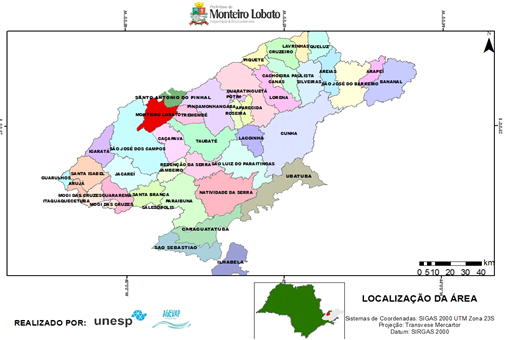
\includegraphics[width=1\linewidth]{produtos/proddois/image16}
	\caption{Divisão territorial dos municípios da RMVP}
	\legend{Fonte: IBGE, 2010 e EMPLASA, 2017}
	\label{fig:image16}
\end{figure}

O município faz divisa com os municípios de Sapucaí-Mirim (MG) e Santo Antônio do Pinhal (SP), ao norte; São José dos Campos e Caçapava, ao sul; com Taubaté e Tremembé, a leste; e com São Francisco Xavier, distrito de São José dos Campos, a oeste, como demonstrado na \autoref{fig:image17}. Tem como principais acessos, partindo de São Paulo, pelas rodovias BR-116 (Rodovia Presidente Dutra) ou pela SP-70 (Rodovia Carvalho Pinto) e posteriormente pela SP-50 (São José dos Campos/Campos do Jordão). Cabe destaque a essa última, frente à sua inserção na malha urbana de Monteiro Lobato ~\cite{MonteiroLobatoSite}.

\begin{figure}[h!]
	\centering
	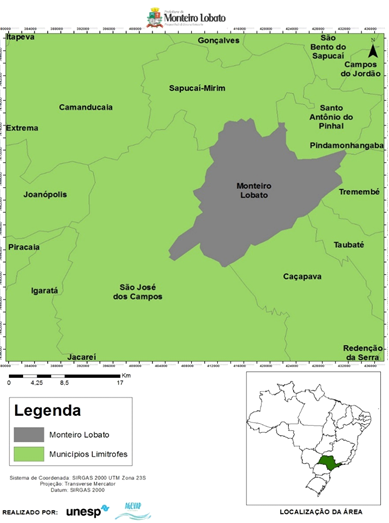
\includegraphics[width=0.9\linewidth]{produtos/proddois/image17}
	\caption{Mapa de localização de Monteiro Lobato no Brasil e no estado de São Paulo. }
	\legend{Fonte: IBGE, 2010}
	\label{fig:image17}
\end{figure}

\subsection{Bacia hidrográfica do rio Paraíba do Sul}
O município de Monteiro Lobato está inserido na bacia do rio Paraíba do Sul, que possui uma área de drenagem de 61.307 km² distribuída pelos estados de São Paulo (SP) (13.934 km²), Rio de Janeiro (RJ) (26.674 km²) e Minas Gerais (MG) (20.699 km²) (CEIVAP, AGEVAP, COHIDRO, 2014a) . 

O Rio Paraíba do Sul é formado pela união dos rios Paraibuna e Paraitinga, na Serra da Bocaina, Estado de São Paulo, e sua foz encontra-se no município de São João da Barra, no Estado do Rio de Janeiro, a mais de mais de 1.100 km de suas nascentes. A bacia drena uma das regiões mais desenvolvidas do país, abrangendo parte do Estado de São Paulo, na região conhecida como Vale do Paraíba Paulista, parte do Estado de Minas Gerais, denominada Zona da Mata Mineira, e metade do Estado do Rio de Janeiro. A bacia abrange 184 municípios, 36 dos quais estão parcialmente inseridos na bacia. A população  total da bacia é 7,28 milhões de habitantes, dos quais 38\% (2,79 milhões) em SP, 39\% (2,86 milhões) no RJ e 22\% (1,63 milhão) em MG. O Sistema Hidráulico do Rio Paraíba do Sul, um complexo conjunto de reservatórios e estruturas hidráulicas existentes nas bacias hidrográficas do Paraíba do Sul e do Guandu, no Rio de Janeiro, é o responsável por reservar e transportar dois terços da vazão do Rio Paraíba do Sul para a bacia do Guandu, com o objetivo de gerar energia elétrica e garantir o abastecimento de cerca de nove milhões de pessoas na Região Metropolitana do Rio de Janeiro (KUMLER; LEMOS, 2008; ANA, 2015). Entre as décadas de 1930 a 1960 foram construídas as principais barragens ao longo do rio, quais sejam: Paraibuna/Paraitinga, Santa Branca, Funil, Santa Cecília e Ilha dos Pombos ~\cite{ANA2017}.

Deve-se destacar que o Sistema Hidráulico do Rio Paraíba do Sul é responsável por suprir de energia elétrica e água a cidade do Rio de Janeiro. Este sistema se subdivide em dois subsistemas:

Paraíba: compreende a transposição das águas do rio Paraíba do Sul em Santa Cecília. Esse subsistema é composto pela estação elevatória de Santa Cecília, barragem de Santana, estação elevatória de Vigário, usinas hidrelétricas Nilo Peçanha e Fontes Nova, reservatório de Ponte Coberta e usina hidrelétrica Pereira Passos;
Lajes: consiste das barragens de Tocos e Lajes, calha da CEDAE e das Usinas Fontes Nova e Fontes Velha (está atualmente desativada).

\section{Histórico}

O nome do município Monteiro Lobato é uma referência ao escritor José Bento de Monteiro Lobato, reconhecido nacionalmente por sua influência na cultura do país. A região foi onde o escritor viveu e, em uma fazenda denominada “Fazenda do Visconde”, obteve inspiração para criar muitas de suas obras, incluindo muitos dos elementos que compuseram o ícone cultural de histórias infantis “Sítio do Pica-Pau Amarelo” ~\cite{squeff2003origem,IBGE2010}. As Figuras \ref{fig:image18} e \ref{fig:image19} mostram a fazenda em que o escritor viveu. 
 
\begin{figure}[h!]
	\centering
	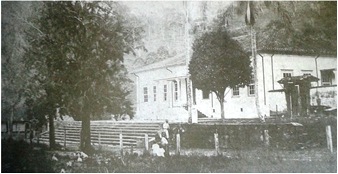
\includegraphics[width=0.8\linewidth]{produtos/proddois/image18}
	\caption{Fachada da frente da casa “Fazenda do Visconde”.}
	\legend{Fonte: Retirado do Site "O verdadeiro Sítio do Picapau Amarelo."}
	\label{fig:image18}
\end{figure}

\begin{figure}[h!]
	\centering
	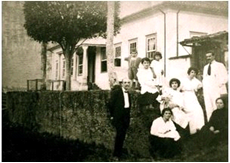
\includegraphics[width=0.8\linewidth]{produtos/proddois/image19}
	\caption{Monteiro Lobato ainda criança em frente ao casarão da fazenda em que morava.}
	\legend{Fonte: Arquivo Pessoal/André Barreto.}
	\label{fig:image19}
\end{figure}

Segundo a Prefeitura de Monteiro Lobato, antes deste nome, a localidade que era incluída dentro dos limites do município de Taubaté, e possuiu quatro nomes: Freguesia das Estacas, Freguesia de Nossa Senhora do Bonsucesso do Buquira, Vila das Palmeiras do Buquira e Vila do Buquira ~\cite{MonteiroLobatoSite}. Entretanto, era comumente denominada apenas como Buquira, que em tupi-guarani significa “Ribeirão dos Pássaros”, por situar-se à uma das margens do rio Buquira ~\cite{IBGE2010}.

Em 1857, Buquira foi denominada como Freguesia e Distrito de Paz até que em 1900 ascendeu à condição de Vila. Em 1934 ascendeu a cidade, por lei estadual, entretanto no mesmo ano, ainda com a nomenclatura de Buquira, foi reduzida à condição de distrito e incluída ao município de São José dos Campos, até ser emancipada em 1948 para então, um ano depois, receber o atual nome ~\cite{MonteiroLobatoSite}.

A história do município está inserida no contexto do Vale do Paraíba como caminho dos bandeirantes e dos tropeiros, participando também dos ciclos econômicos do café e da pecuária leiteira. Houve, no município, períodos de prosperidade que foram seguidos de períodos de estagnação econômica, provocando assim, o êxodo de parte de sua população ~\cite{MonteiroLobato2014}.

O movimento da Rodovia Monteiro Lobato (SP-50), que liga São José dos Campos a Campos do Jordão, contribuía para o pequeno comércio local com as paradas dos viajantes que, mesmo em curto período de tempo, consumiam produtos característicos da cidade. Entretanto, com a construção da Rodovia Floriano Rodrigues Pinheiro (SP-123) em 1978, ligando Taubaté a Campos do Jordão, Monteiro Lobato teve sua economia novamente prejudicada ~\cite{MonteiroLobato2014}.

Por outro lado, embora estrategicamente localizado no caminho para São Francisco Xavier, distrito de São José dos Campos, e para Campos do Jordão e sul de Minas Gerais, seu desenvolvimento econômico lento colaborou para o que hoje são os seus maiores atrativos turísticos: a preservação de 50,80\% da vegetação do município e suas características de uma pequena cidade rural com vida tranquila ~\cite{MonteiroLobato2014}.

\section{Turismo, cultura e lazer}

De acordo com o artigo 2º da Lei N° 11.771, de 17 de setembro de 2008, que dispõe sobre a Política Nacional de Turismo e dá outras providências, é considerado turismo as atividades realizadas por pessoas físicas durante viagens e estadias em lugares diferentes do seu entorno habitual, por um período inferior a 1 (um) ano, com finalidade de lazer, negócios ou outras.
No Brasil, a participação direta do turismo na economia foi de US\$ 56,8 bilhões em 2016, o equivalente a 3,2\% do PIB. Já a contribuição total do setor foi de US\$ 152,2 bilhões, 8,5\% do PIB Nacional. Segundo dados da World Travel \& Tourism Council (WTTC), o setor de turismo gerou mais de 7 milhões de empregos em 2016, o que representa 7,8\% do total de empregos. Estão incluídas, como geradoras de empregos diretos, as atividades relacionadas a hotelaria, agências de turismo, companhias aéreas, demais tipos de transportes de passageiros e turistas, além de restaurantes e empreendimentos de lazer ~\cite{PNT2018}.

O município de Monteiro Lobato conta com um Plano Diretor de Turismo Sustentável de Monteiro Lobato (P), elaborado pelo Grupo de Planejamento Participativo do Turismo Sustentável de Monteiro Lobato (PlaneJÁtur). Como um documento complementar, há um Plano de Desenvolvimento Turístico Municipal de Monteiro Lobato (PDTM) elaborado por uma parceria entre o curso de Turismo na Universidade de São Paulo (USP) e a Prefeitura Municipal de Monteiro Lobato, iniciado em 2013.

A cidade possui diversos monumentos, construções e manifestações culturais que podem ser considerados patrimônio histórico cultural da cidade. Os mesmos são registros da cultura, tradições e/ou história local e se mostram de extrema importância para manter a identidade do município (PDTM, 2013).

A Igreja Matriz, por exemplo, simboliza a origem do município, pois foi a partir dela que houve o surgimento da Freguesia, que, futuramente, viria a se transformar no Município de Monteiro Lobato. A arquitetura da cidade, principalmente na região central, manteve-se, em sua maior parte, preservada, o que contribuiu para a manutenção da identidade do município e também se alia aos seus aspectos imateriais, caracterizados por seus saberes locais, suas festas tradicionais e populares, além do ambiente de tranquilidade e com características caipiras ainda preservados na cidade (PDTM, 2013).

A maior influência cultural e artística do município se dá pelos contos do Sítio do Pica-Pau Amarelo, escritos por José Bento Monteiro Lobato, no período em que viveu no local e deu início à essa obra literária de grande relevância na Literatura Infantil Brasileira. O casarão onde o escritor morou é aberto ao público e administrado por Maria Lucia Ribeiro, o sítio lobatense conta com dezoito cômodos compostos por bibliotecas e mobília do início século passado. Além do casarão como construção principal, a propriedade possui uma extensa área verde e uma cachoeira conhecida como “Reino das Águas Claras”, batizada pelo próprio Lobato.

Os contos do Sítio do Pica-Pau Amarelo acarretam, atualmente, na propagação de diversas lendas no cotidiano do lobatense, desde personagens folclóricos como o Saci e criaturas da mitologia. Além disso, disseminam o artesanato local como bonecas da personagem Emília e outros presentes na obra; tanto quanto o comércio e a infraestrutura local como nomes de restaurantes e escolas.

Desde o ano de 2010, acontece no município o Festival de Literatura Infantil, sempre no mês de setembro com todas as atividades gratuitas. Com o objetivo de preservar a memória do escritor José Bento Monteiro Lobato, incentivar a leitura e formar novos leitores. As figuras \ref{fig:image20}, \ref{fig:image21} e \ref{fig:image22} mostram alguns registros fotográficos do Festival.
 
 \begin{figure}[h!]
 	\centering
 	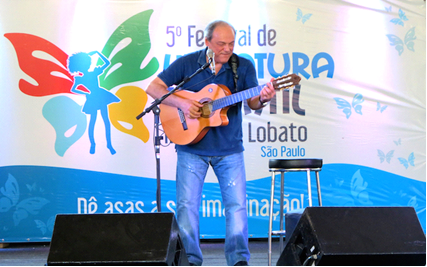
\includegraphics[width=0.85\linewidth]{produtos/proddois/image20}
 	\caption{Festival de Literatura Infantil em Monteiro Lobato de 2014 – Parte I.}
 	\legend{Fonte: Prefeitura de Monteiro Lobato.}
 	\label{fig:image20}
 \end{figure}

 \begin{figure}[h!]
 	\centering
 	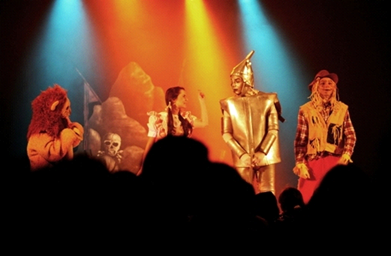
\includegraphics[width=0.85\linewidth]{produtos/proddois/image21}
 	\caption{Festival de Literatura Infantil em Monteiro Lobato de 2014 – Parte II.}
 	\legend{Fonte: Prefeitura de Monteiro Lobato.}
 	\label{fig:image21}
 \end{figure}

 \begin{figure}[h!]
	\centering
	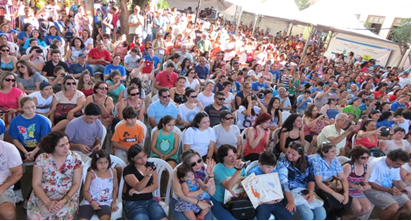
\includegraphics[width=0.85\linewidth]{produtos/proddois/image22}
	\caption{Festival de Literatura Infantil em Monteiro Lobato de 2014 – Parte III.}
	\legend{Fonte: Prefeitura de Monteiro Lobato.}
	\label{fig:image22}
\end{figure}

Outros festivais, manifestações e tradições culturais de alto impacto no munícipio são os Pereirões, os Grupos Moçambique Esperança e Catira União Lobatentes (grupos dançantes). Os Pereirões são bonecos gigantes associados à época de Carnaval, possuem corpos de jacá, um cesto feito de bambu e cipó e altura superior a três metros, como mostra a \autoref{fig:image23}. A estrutura é carregada pelos foliões durante a celebração, que realizam danças, giros e corridas com o público.


 \begin{figure}[!h]
	\centering
	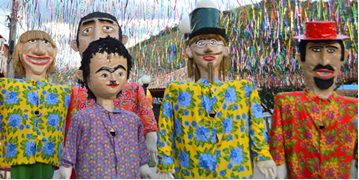
\includegraphics[width=0.85\linewidth]{produtos/proddois/image23}
	\caption{Pereirões de Monteiro Lobato.}
	\legend{Fonte: Prefeitura de Monteiro Lobato.}
	\label{fig:image23}
\end{figure}

O Grupo Catira surgiu da década de 1930 pelos irmãos Francisco Rosa e Antônio Rosa, e é marcado por passos firmes e palmas sincronizadas, ritmo composto pelo som da viola caipira, entoado por dois violeiros. A dança é executada em duas fileiras – uma em frente à outra, formando pares. O chapéu é uma peça fundamental. O Grupo Moçambique Esperança é um grupo que repercute uma dança de origem africana e que chegou ao município no ano de 1940. Com movimentos ritmados, produz belos efeitos sonoros. Utilizam bastões que servem para marcar o ritmo da dança, além de instrumentos de percussão e corda. Os grupos supracitados são mostrados na \autoref{fig:image24} e \autoref{fig:image25} respectivamente.


 \begin{figure}[h!]
	\centering
	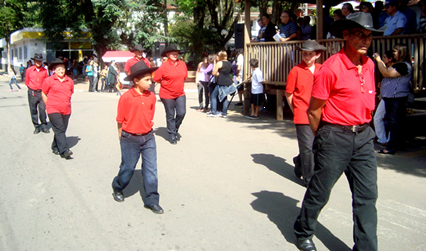
\includegraphics[width=0.85\linewidth]{produtos/proddois/image24}
	\caption{Grupo Catira de Monteiro Lobato.}
	\legend{Fonte: Prefeitura de Monteiro Lobato.}
	\label{fig:image24}
\end{figure}

 \begin{figure}[h!]
	\centering
	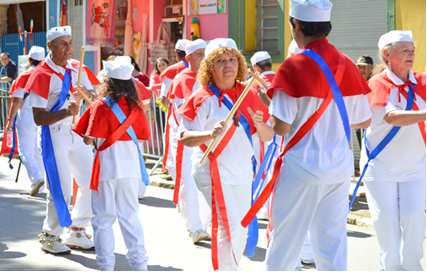
\includegraphics[width=0.85\linewidth]{produtos/proddois/image25}
	\caption{Grupo Moçambique Esperança.}
	\legend{Fonte: Prefeitura de Monteiro Lobato.}
	\label{fig:image25}
\end{figure}

Ademais, o município tem fortes influências da Igreja Católica e possui diversas festas religiosas que acontecem no decorrer do ano. No mês de janeiro acontecem homenagens a São Sebastião; no mês de maio, Santa Rita de Cássia é venerada no bairro do Souza; e em setembro ocorre a comemoração em torno da padroeira, Nossa Senhora de Bonsucesso. 

\section{Geografia física}

A geografia física corresponde ao meio de suporte sobre o qual se desenvolve tanto o meio biótico, objeto do próximo item, como o meio antrópico. Os temas a serem abordados correspondem ao solo, água e ar, mas são aqui tratados dentro de uma perspectiva que objetiva descrever as características locacionais do município para potenciais infraestruturas de gestão de Resíduos Sólidos. Os dados aqui apresentados foram coletados e produzidos pelo Instituto de Pesquisas Tecnológicas - IPT no ano de 2016, como parte do diagnóstico de base para o novo Plano Diretor para a cidade de Monteiro Lobato.

\subsection{Clima}

A classificação climática de Köppen é uma classificação baseada no pressuposto de que a vegetação natural é a melhor expressão do clima de uma região e as modificações críticas ao sistema são sempre relacionadas aos limites térmicos/hídricos dos tipos de climas determinados para diferentes regiões. Assim, as fronteiras entre regiões climáticas foram selecionadas para corresponder, tanto quanto possível, às áreas de predominância de cada tipo de vegetação, razão pela qual a distribuição global dos tipos climáticos e a distribuição dos biomas apresenta elevada correlação ~\cite{Rolim2007}. Segundo essa classificação, Monteiro Lobato possui clima do tipo Cwa, considerado um clima temperado úmido com Inverno seco e Verão quente. Com temperatura média anual de 20,9°C, oscilando entre mínima média de 14,6°C e máxima média de 27,2°C.

A precipitação média total anual é de 1870,4 mm. A \autoref{fig:image26} mostra o panorama da precipitação média mensal, entre 1939 e 2004, onde é possível observar a distribuição da precipitação ao longo do ano, com destaque para o período de inverno seco, descrito anteriormente ~\cite{MonteiroLobato2014}.

 \begin{figure}[h!]
	\centering
	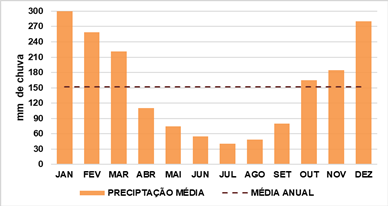
\includegraphics[width=1\linewidth]{produtos/proddois/image26}
	\caption{Precipitações médias mensais no período de 1939 a 2004.}
	\legend{Fonte: ~\cite{MonteiroLobato2014}.}
	\label{fig:image26}
\end{figure}

\subsection{Geologia}

O município de Monteiro Lobato é formado pelas seguintes unidades geológicas: Complexo Embu, Complexo Varginha-Guaxupé, depósitos aluvionares, Formação Boturana e maciços graníticos, além de falhas geológicas. O Complexo Embu é formado por xistos, filitos, migmatitos, gnaisses migmatizados e corpos lenticulares de quartzitos, anfibolitos e rochas calciossilicatadas e possui afloramentos com direção NE-SW. Já o Complexo de Varginha-Guaxupé é formado por gnaisses neoproterozóicos, de origem ígnea e sedimentar. Este complexo é dividido em três unidades: Granulítica Basal, Ortognáissica Migmatítica Intermediária e Paragnáissica Migmatítica Superior.  Ao menos as duas unidades superiores são intrudidas por um granitóide cedo a sin-colisional que ocorre restrito ao domínio do Complexo Varginha-Guaxupé. A Formação Boturuna é formada pormetapelitos com lentes de quartzitos na base e rochas carbonáticas no topo. Os depósitos aluvionares, por sua vez, são formados por depósitos sedimentares gerados pelo transporte de material realizado pelas águas correntes ~\cite{CPRM}.

A \autoref{fig:image27} mostra as unidades geológicas distribuídas pelo território do município de Monteiro Lobato. Através dela, pode-se perceber que as unidades geológicas predominantes são o Complexo de Embu e o Complexo de Varginha-Guaxupé.
\clearpage
\begin{figure}[h!]
	\centering
	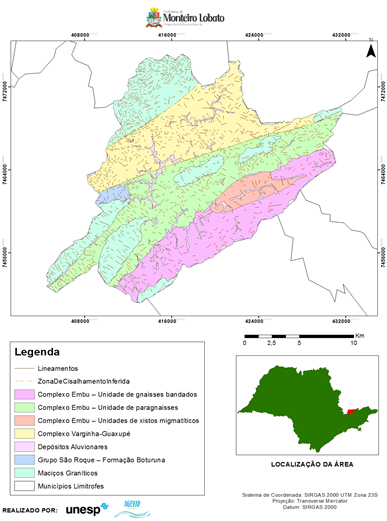
\includegraphics[width=1\linewidth]{produtos/proddois/image27}
	\caption{Unidades geológicas do Município de Monteiro Lobato.}
	\legend{Fonte: Adaptado IPT, 2016.}
	\label{fig:image27}
\end{figure}

\subsection{Geomorfologia}

Segundo Ab’Sáber (2007), Monteiro Lobato está situada no domínio morfoclimático tropical-atlântico, chamado de “mares de morros” florestados. Esse domínio apresenta a seguinte combinação de fatos fisiográficos: decomposição funda e universal das rochas cristalinas ou cristalofilianas, de 3 a 5 até 40 a 60 m de profundidade; presença de solo de tipo latossolo ou pedosolo amarelo-vermelho; superposição de solos devido às flutuações climáticas finais do quaternário em sertões sincopados; mamelonização universal das vertentes, desde o nível de morros altos até os níveis dos morros intermediários e patamares de relevo; drenagem originalmente perene até para o menor dos ramos das redes hidrográficas dendríticas regionais; lençol d’água subterrâneo que alimenta permanentemente, durante e entre as chuvas, a correnteza dos leitos dos cursos d’água; forte cota de umidade do ar; equilíbrio sutil entre processos morfoclimáticos, pedológicos, hidrológicos e ecossistêmicos.

A paisagem natural é o resultado de diferentes elementos que compõem o meio físico como rocha, relevo, solo e vegetação. Neste contexto, a compreensão e a identificação das diferentes formas de relevo se constituem componente de grande importância na implantação de qualquer atividade antrópica que altere significativamente a paisagem. O município de Monteiro Lobato se localiza em um território com colinas, escarpas, morros altos, morros baixos, morrotes, serras, planícies e terraços fluviais. Entretanto, de acordo com o Plano Diretor do Turismo Sustentável de Monteiro Lobato (2014), 59,72\% da área do município está entre as cotas altimétricas de 700 a 1.000 m, que representam a transição entre o relevo de morros e as escarpas da Serra da Mantiqueira. As maiores altitudes aparecem ao norte do município na divisa com o município de Santo Antônio do Pinhal e na divisa com o Estado de Minas Gerais. As menores altitudes estão associadas ao sul do município e às várzeas dos rios Ferrão ou Buquira e Buquirinha \autoref{fig:image28}. 

Essa configuração de relevo pode propiciar o aparecimento de fenômenos naturas de movimentos de massa, o que inclui escorregamentos, quedas de blocos e rastejos (movimentos lentos nos solos). Nestas áreas de concentração, os principais fragmentos de floresta têm um importante papel na perenização das nascentes, na infiltração da água no solo e na regulação do escoamento de base. Com a remoção destas florestas, as áreas de serras e escarpas passam a funcionar, hidrologicamente, como áreas com grande volume e elevada velocidade do escoamento superficial \textbf{(>SIMÕES, 2012).}
\clearpage
 \begin{figure}[h!]
 	\centering
 	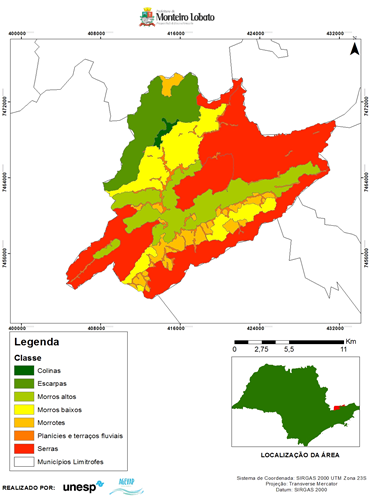
\includegraphics[width=1\linewidth]{produtos/proddois/image28}
 	\caption{Unidades geomorfológicas no munício de Monteiro Lobato -SP.}
 	\legend{Fonte: Adaptado IPT, 2016.}
 	\label{fig:image28}
 \end{figure}

\subsection{Relevo}

Monteiro Lobato está localizada nas escarpas e reversos da Serra da Mantiqueira, apresentando uma topografia montanhosa. A área urbana está a 650 m de altitude em relação ao nível do mar. Por esses fatores, a declividade no munícipio é um elemento decisivo que interfere de forma significativa na distribuição de classes de solos, bem como exerce influência nos processos de erosão, exigindo manejos agrícolas diferenciados para uma ocupação adequada das terras ~\cite{MonteiroLobato2014}.

A \autoref{fig:image29} nos permite aferir que as declividades menores estão   associadas às áreas de várzeas dos rios Buquira/Ferrão e Buquirinha. Ela mostra também como a declividade média de Monteiro Lobato varia entre 17-20º, sendo que em sua maioria, o munícipio apresenta áreas bastante declinosas (>20º).
\clearpage
\begin{figure}[h]
	\centering
	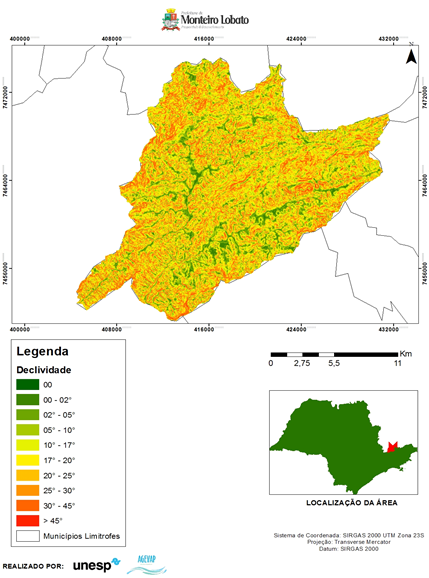
\includegraphics[width=1\linewidth]{produtos/proddois/image29}
	\caption{Declividade do município de Monteiro Lobato -SP.}
	\legend{Fonte: Adaptado IPT, 2016.}
	\label{fig:image29}
\end{figure}

\subsection{Recursos naturais}

Em Monteiro Lobato, o tipo de vegetação predominante é a Floresta Ombrófila Densa, cuja característica mais marcante é a presença de árvores altas, atingindo entre 20 e 30 m.  Estas árvores possuem folhas largas e sempre verdes de longa duração (perenifólias), além de mecanismos adaptados para resistir tanto a períodos de calor extremo, quanto de muita umidade. Entretanto, a cobertura vegetal natural não se encontra mais em seu estado original, pois delas já foram removidas as árvores de grande porte fornecedoras de madeira. Mesmo assim, Monteiro Lobato preserva 50,80\% de sua vegetação nativa, somando 16.912 hectares ~\cite{MonteiroLobato2014}.

O município possui em seu território parte de uma unidade de conservação de uso sustentável, a Área de Preservação Ambiental (APA) da Bacia do Rio Paraíba do Sul, além da Reserva Particular de Patrimônio Natural (RPPN) Sítio do Cantoneiro (Figura 15), que contribuem para a manutenção da vegetação natural restante no município. 

No estudo produzido por Arcorverde 2018, que ranqueia os municípios da região metropolitana do Vale do Paraíba e Litoral Norte do estado de São Paulo, com uma faixa entre 0 e 1 para os desempenhos Ambientais, socioeconômico e institucional, posicionou Monteiro Lobato como o 10° município entre os 39 avaliados.   Dentre os índices de desempenho, Monteiro Lobato foi ranqueado com 0,60 para ambiental, 0,33 para socioeconômico e 0,1 para institucional ~\cite{arcoverdeproposiccao} aproximadamente. 

 Figura 15. Recurso naturais do município de Monteiro Lobato -SP.
Fonte: Adaptado IPT, 2016.

\subsection{Hidrografia}

A UGRHI  02 – Paraíba do Sul é constituída pela Bacia do Rio Jaguari e de outros tributários do Rio Paraíba do Sul, tanto da margem esquerda como da direita, desde as nascentes de seus formadores (rios Paraibuna e Paraitinga) até a divisa dos Estados de São Paulo e do Rio de Janeiro, a montante da barragem do Funil. Em condições naturais, a UGRHI - 02 não recebe contribuições nem deságua em outras bacias hidrográficas do Estado de São Paulo. Os principais afluentes do Rio Paraíba do Sul no seu trecho paulista são: o Paraibuna, o Paraitinga, o Jaguari, o Una, o Buquira/Ferrão, o Embaú/Piquete, o Bocaina e o Pitangueiras/Itagaçaba ~\cite{MonteiroLobato2014}.

A sub-bacia do Rio Buquira, no município de Monteiro Lobato, integrada à bacia do Rio Paraíba do Sul, é composta, entre outros, pelos rios Buquira/Ferrão, Braço e Descoberto; pelo córrego do Machado e pelos ribeirões Souzas e Matinada. Monteiro Lobato apresenta uma rede de drenagem densa, o que faz dos recursos hídricos um fator importante para a cidade (Figura 16). Na figura citada entende-se por curso d’água os elementos como: rios, ribeirões, córregos, riachos etc. e, por corpo d’água:  lagos, lagoas, zonas úmidas etc. 


 
Figura 16. Rede de drenagem do município de Monteiro Lobato -SP.
Fonte: Adaptado IPT, 2016.

\section{Organização territorial e político-administrativa}
\subsection{Organização territorial}
\subsubsection{Distritos e Bairros}

No município de Monteiro Lobato não há formação de distritos, possuindo 19 bairros distribuídos por seu território, e listado conforme na \autoref{tab:bairros}.

	% Table generated by Excel2LaTeX from sheet 'bairros_monteiro'
\begin{table}[htbp]
  \centering
  \arrayrulecolor[rgb]{ 1, 1, 1}
  \caption{Bairros de Monteiro Lobato.}
    \begin{tabular}{c|c}
    \rowcolor[rgb]{ .984,  .831,  .706} Bairro do Souza & Bairro da Matinada \\
    \rowcolor[rgb]{ .992,  .914,  .851} Centro & Bairro Pedra Branca \\
    \rowcolor[rgb]{ .984,  .831,  .706} Vila São Sebastião & Bairro da Serrinha \\
    \rowcolor[rgb]{ .992,  .914,  .851} Vila Esperança & Bairro dos Teixeiras \\
    \rowcolor[rgb]{ .984,  .831,  .706} Vargem Alegre & Bairro Ponte Nova \\
    \rowcolor[rgb]{ .992,  .914,  .851} Bairro São Benedito & Bairro do Turvo \\
    \rowcolor[rgb]{ .984,  .831,  .706} Bairro Descoberto & Bairro dos Forros \\
    \rowcolor[rgb]{ .992,  .914,  .851} Jardim Morada do Sol & São Gotardo \\
    \rowcolor[rgb]{ .984,  .831,  .706} Bairro Alpes do Buquira & Bairro Brumado \\
    \rowcolor[rgb]{ .992,  .914,  .851} Bairro Taquari & Bairro Ferreiras \\
    \end{tabular}%
  \label{tab:bairros}%
\end{table}%


\subsection{Organização Político Administrativa}
O Poder Executivo dentro dos limites do município é exercido pelo Prefeito, cujo gabinete está atualmente estruturado conforme a \autoref{tab:gabinete}. A prefeita, primeira mulher a exercer tal cargo, foi eleita em 2012 para exercício em 2013 e reeleita em 2016 para novo exercícios.

	% Table generated by Excel2LaTeX from sheet 'gabinete'
\begin{table}[htbp]
  \centering
  \arrayrulecolor{white}
  \caption{Gabinete da Prefeitura de Monteiro Lobato.}
    \begin{tabular}{P{0.2\textwidth} P{0.4\textwidth} P{0.1\textwidth}}
    \rowcolor[rgb]{ .969,  .588,  .275} 
    \multicolumn{1}{P{0.2\textwidth}}{\textcolor[rgb]{ 1,  1,  1}{\textbf{Cargo}}} & \multicolumn{1}{P{0.4\textwidth}}{\textcolor[rgb]{ 1,  1,  1}{\textbf{Nome do responsável}}} & \textcolor[rgb]{ 1,  1,  1}{\textbf{Partido}} \\
    \rowcolor[rgb]{ .992,  .914,  .851} Prefeita & Daniela de Cássia Santos Brito & PSB \\
    \rowcolor[rgb]{ .984,  .831,  .706} Vice-Prefeito & Vicente de Paula Prisco da Cunha & PSDB \\
    \end{tabular}%
  \label{tab:gabinete}%
\end{table}%



O gabinete é auxiliado pelos Secretários Municipais, os quais são divididos em 9 secretarias, como mostra a \autoref{tab:secretarias} com seus respectivos representantes. A Secretaria Municipal de Administração é o órgão da estrutura organizacional da Prefeitura incumbido de desempenhar atividades pertinentes às áreas de recursos humanos, compras e licitações, segurança do trabalho, tecnologia da informação e protocolo (abertura e acompanhamento de processos) ~\cite{MonteiroLobatoSite}.

A Secretaria de Cultura e Turismo planeja e coordena o apoio e a execução de atividades para a difusão e formação cultural, bem como a valorização das raízes culturais da população e o desenvolvimento da cidadania no município de Monteiro Lobato. A Secretaria de Cultura e Turismo é responsável pela organização das festas tradicionais e dos eventos de caráter cultural do município lobatense ~\cite{MonteiroLobatoSite}.

A Secretaria Municipal de Desenvolvimento Social de Monteiro Lobato tem por objetivo formular, implantar, financiar, executar, monitorar e avaliar a Política Municipal de Assistência Social, como parte integrante do Sistema Único de Assistência Social (SUAS). As políticas públicas implantadas na Secretaria visam prestar o atendimento integral às famílias, as crianças e aos adolescentes, as mulheres, aos idosos e as pessoas portadoras de necessidades especiais, sendo que a maior prioridade são os segmentos em situação de maior vulnerabilidade social ~\cite{MonteiroLobatoSite}.
A Secretaria Municipal de Educação tem como objetivo principal trabalhar com a ideia de Inclusão em todos os níveis, integrando cooperativamente todas as escolas do município, sejam elas municipais, estaduais ou privadas ~\cite{MonteiroLobatoSite}.

A Secretaria de Esportes e Lazer trabalha para oferecer à população opções nas áreas de esportes e entretenimento, de forma gratuita. Além disso, fomenta as atividades de competição envolvendo os moradores de Monteiro Lobato, principalmente a juventude ~\cite{MonteiroLobatoSite}.

A Secretaria de Finanças e Tributação desenvolve as atividades governamentais superiores de condução dos negócios da fazenda pública municipal, em atendimento às diretrizes traçadas pelo chefe do executivo e as atividades administrativas, objetivando a concretização das decisões políticas, principalmente, mas não só apenas, no que tange a elaboração do PPA (Plano Plurianual), da LDO (Lei de Diretrizes Orçamentárias) e da LOA (Lei Orçamentária Anual), isso com o auxílio das demais secretarias e órgãos da Administração Pública, bem como ao que se refere ao planejamento orçamentário, à execução orçamentária, à realização de receitas, a efetivação das despesas, a movimentação financeira e a administração tributária ~\cite{MonteiroLobatoSite}.

É de competência básica da Secretaria Municipal Meio Ambiente e Agricultura o planejamento, apoio e desenvolvimento de políticas públicas para o setor agropecuário e para a conservação e proteção do meio ambiente. Atua no setor de Meio Ambiente, cujo objetivo é gerenciar o ambiente local buscando diminuição de impactos negativos para todas as formas de vida e a conservação dos recursos naturais; e no setor de Agricultura, com o objetivo de incentivar e promover atividades ligadas à agricultura e à pecuária ~\cite{MonteiroLobatoSite}.

O serviço de saúde, de responsabilidade integral da Secretaria Municipal de Saúde, preza pelo bom atendimento dentro das normas preconizadas pelo SUS e objetiva acolher para cuidar, trabalhando na prevenção de doenças e agravos, visando o bem-estar e qualidade de vida das pessoas. Conta com atendimento na zona urbana e nos bairros da zona rural, com duas equipes compostas com médico, enfermeira, auxiliar de enfermagem e agente comunitário de saúde ~\cite{MonteiroLobatoSite}.

Já a Secretaria Municipal de Transportes tem a função de manter as estradas rurais em boas condições de tráfego. O município tem quase 400 km de estradas que levam a diversos bairros na zona rural. Este cuidado se justifica pela vocação rural de Monteiro Lobato, o que exige estradas bem cuidadas para facilitar o transporte de produtos agropecuários, especialmente a produção de leite ~\cite{MonteiroLobatoSite}.

%	% Table generated by Excel2LaTeX from sheet 'secretarias'
\begin{table}[htbp]
	\centering
	\caption{Secretarias Municipais de Monteiro Lobato.}
	\begin{tabular}{c|c}
		\rowcolor[rgb]{ .969,  .588,  .275} \textcolor[rgb]{ 1,  1,  1}{\textbf{Divisão}} & \textcolor[rgb]{ 1,  1,  1}{\textbf{Nome do responsável}} \\
		\rowcolor[rgb]{ .992,  .914,  .851} Administração & Priscila Maria Medeiros Dias Magalhães \\
		\rowcolor[rgb]{ .984,  .831,  .706} Cultura e Turismo & Mariana Santos \\
		\rowcolor[rgb]{ .992,  .914,  .851} Desenvolvimento Social & Alexandre Nunes Barbedo \\
		\rowcolor[rgb]{ .984,  .831,  .706} Educação & Ellen Denise Dias da Silva Veloso Bertolini \\
		\rowcolor[rgb]{ .992,  .914,  .851} Esportes e Lazer & Tiago Viana \\
		\rowcolor[rgb]{ .984,  .831,  .706} Finanças e Tributação & Nayane Larissa Rocha Silva \\
		\rowcolor[rgb]{ .992,  .914,  .851} Meio Ambiente e Agricultura & Pedro Luiz de Souza Morais \\
		\rowcolor[rgb]{ .984,  .831,  .706} Saúde & Cláudia Mara Darrigo \\
		\rowcolor[rgb]{ .992,  .914,  .851} Transportes e Serviços Gerais & Aluani Sene \\
	\end{tabular}%
	\label{tab:secretarias}%
\end{table}%


% Table generated by Excel2LaTeX from sheet 'secretarias'
\begin{table}[htbp]
	\centering
	\caption{Secretarias Municipais de Monteiro Lobato.}
	\begin{tabular}{c|c}
		\rowcolor[rgb]{ .969,  .588,  .275} \textcolor[rgb]{ 1,  1,  1}{\textbf{Divisão}} & \textcolor[rgb]{ 1,  1,  1}{\textbf{Nome do responsável}} \\
		\rowcolor[rgb]{ .992,  .914,  .851} Administração & Priscila Maria Medeiros Dias Magalhães \\
		\rowcolor[rgb]{ .984,  .831,  .706} Cultura e Turismo & Mariana Santos \\
		\rowcolor[rgb]{ .992,  .914,  .851} Desenvolvimento Social & Alexandre Nunes Barbedo \\
		\rowcolor[rgb]{ .984,  .831,  .706} Educação & Ellen Denise Dias da Silva Veloso Bertolini \\
		\rowcolor[rgb]{ .992,  .914,  .851} Esportes e Lazer & Tiago Viana \\
		\rowcolor[rgb]{ .984,  .831,  .706} Finanças e Tributação & Nayane Larissa Rocha Silva \\
		\rowcolor[rgb]{ .992,  .914,  .851} Meio Ambiente e Agricultura & Pedro Luiz de Souza Morais \\
		\rowcolor[rgb]{ .984,  .831,  .706} Saúde & Cláudia Mara Darrigo \\
		\rowcolor[rgb]{ .992,  .914,  .851} Transportes e Serviços Gerais & Aluani Sene \\
	\end{tabular}%
	\label{tab:secretarias}%
\end{table}%


\subsubsection{Poder Legislativo}
O Poder Legislativo é exercido pela Câmara dos Vereadores, e é composta em Monteiro Lobato por 9 vereadores, como previsto para Municípios de até 15.000 (quinze mil) habitantes – no Capítulo IV, artigo 29 da Constituição Federal de 1988. A Mesa Diretora é composta pelo Presidente, Vice-Presidente, Primeiro Secretário e Segundo Secretário.

De acordo com o Artigo 21 do Regimento Interno da Câmara Municipal de Monteiro Lobato, o Presidente é o representante legal da Câmara em suas relações externas, cabendo-lhe as funções administrativas de todas as atividades internas, competindo-lhe privativamente as atividades legislativas e a administração das sessões. Ao Primeiro Secretário, cabe constar a presença dos vereadores, assinar (conjuntamente com o Presidente) todas as Atas aprovadas, redigir as Atas das deliberações secretas e auxiliar a Presidência.

Para suprir a falta ou impedimento do Presidente e do Secretário, haverá um Vice-Presidente e um Segundo Secretário, eleitos conjuntamente com aqueles. A formação atual da Mesa Diretora e os demais vereadores encontra-se na \autoref{tab:mesa}, em conjunto com os seus respectivos partidos de posição.

%	% Table generated by Excel2LaTeX from sheet 'mesa_diretora'
\begin{table}[htbp]
	\centering
	\caption{Câmara Municipal - Mesa Diretora e Vereadores de Monteiro Lobato 2019.}
	\begin{tabular}{P{3cm}P{5cm}P{3cm}}
		\rowcolor[rgb]{ .969,  .588,  .275} 
		\multicolumn{1}{P{3cm}}{\textcolor[rgb]{ 1,  1,  1}{\textbf{Cargo}}} & \multicolumn{1}{P{5cm}}{\textcolor[rgb]{ 1,  1,  1}{\textbf{Nome do responsável}}} & \textcolor[rgb]{ 1,  1,  1}{\textbf{Partido}} \\
		\rowcolor[rgb]{ .992,  .914,  .851} 
		\multicolumn{1}{P{3cm}}{Presidente da Câmara} & Carlos Renato Prince & PV \\
		\rowcolor[rgb]{ .984,  .831,  .706} 
		\multicolumn{1}{P{3cm}}{Vice-presidente} & Ailton Rodolfo Martins & PR \\
		\rowcolor[rgb]{ .992,  .914,  .851} 
		\multicolumn{1}{P{3cm}}{Primeira Secretária} & Luis Carlos Diniz & PV \\
		\rowcolor[rgb]{ .984,  .831,  .706} 
		\multicolumn{1}{P{3cm}}{Segundo Secretário} & João Cunha Francisco da Silva & PV \\
		\rowcolor[rgb]{ .992,  .914,  .851} 
		\multicolumn{1}{c}{\multirow{5}{*}{Vereadores}} & Gislene Aparecida Barreto Costa & PSB \\
		\rowcolor[rgb]{ .992,  .914,  .851}       & Jesse Marcos de Azevedo & PV \\
		\rowcolor[rgb]{ .992,  .914,  .851}       & Odair José de Araújo & DEM \\
		\rowcolor[rgb]{ .992,  .914,  .851}       & José Donizeti Pereira & PTB \\
		\rowcolor[rgb]{ .992,  .914,  .851}       & Odair José Rocha & PMDB \\
	\end{tabular}%
	\label{tab:mesa}%
\end{table}%

% Table generated by Excel2LaTeX from sheet 'mesa_diretora'
\begin{table}[htbp]
	\centering
	\caption{Mesa Diretora e Vereadores de Monteiro Lobato 2019.}
	\begin{tabular}{c|p{16.285em}|p{6.785em}}
		\rowcolor[rgb]{ .969,  .588,  .275} \multicolumn{3}{p{35.215em}}{\textcolor[rgb]{ 1,  1,  1}{CÂMARA MUNICIPAL – PODER LEGISLATIVO}} \\
		\rowcolor[rgb]{ .969,  .588,  .275} \multicolumn{1}{p{12.145em}}{\textcolor[rgb]{ 1,  1,  1}{\textbf{Cargo}}} & \multicolumn{1}{p{16.285em}}{\textcolor[rgb]{ 1,  1,  1}{\textbf{Nome do responsável}}} & \textcolor[rgb]{ 1,  1,  1}{\textbf{Partido}} \\
		\rowcolor[rgb]{ .992,  .914,  .851} \multicolumn{1}{p{12.145em}|}{Presidente da Câmara} & Carlos Renato Prince & PV \\
		\rowcolor[rgb]{ .984,  .831,  .706} \multicolumn{1}{p{12.145em}|}{Vice-presidente} & Ailton Rodolfo Martins & PR \\
		\rowcolor[rgb]{ .992,  .914,  .851} \multicolumn{1}{p{12.145em}|}{Primeira Secretária} & Luis Carlos Diniz & PV \\
		\rowcolor[rgb]{ .984,  .831,  .706} \multicolumn{1}{p{12.145em}|}{Segundo Secretário} & João Cunha Francisco da Silva & PV \\
		\rowcolor[rgb]{ .992,  .914,  .851} \multicolumn{1}{c|}{\multirow{5}[0]{*}{Vereadores}} & Gislene Aparecida Barreto Costa & PSB \\
		\rowcolor[rgb]{ .992,  .914,  .851}       & Jesse Marcos de Azevedo & PV \\
		\rowcolor[rgb]{ .992,  .914,  .851}       & Odair José de Araújo & DEM \\
		\rowcolor[rgb]{ .992,  .914,  .851}       & José Donizeti Pereira & PTB \\
		\rowcolor[rgb]{ .992,  .914,  .851}       & Odair José Rocha & PMDB \\
	\end{tabular}%
	\label{tab:mesa}%
\end{table}%


\subsection{Dispositivos legais de zoneamento urbano, disciplinadores do uso e ocupação do solo}
O Plano Diretor é uma lei municipal que estabelece diretrizes para a ocupação da cidade, estabelece as exigências fundamentais de ordenamento da Cidade com o principal objetivo de programar o pleno desenvolvimento de suas funções sociais e garantir o bem-estar de seus habitantes. É instrumento básico e estratégico de desenvolvimento do Município, com ênfase na estruturação do seu território.
No Município de Monteiro Lobato, o Plano Diretor é dado pela Lei Nº 1.650 de 15 de setembro de 2017, na qual são estabelecidas definições importantes que discorrem sobre o ordenamento no município. A referida lei define os usos e atividades geradoras de incômodo ou de impacto à vizinhança e estabelece critérios para análise do grau de incomodidade no Artigo 40, entre eles, poluição sonora, atmosférica, por resíduos líquidos, por resíduos sólidos, vibração e periculosidade.

Em relação aos Recursos Hídricos, algumas ações são definidas no Artigo 67, como: executar programas integrados de saneamento ambiental buscando evitar o desperdício e a degradação de mananciais; implementar instrumentos de Avaliação Ambiental para fins de avaliação, monitoramento e revisão de políticas que ameacem a produção de água; instituir o Programa de Recuperação Ambiental de Cursos D’água e Fundos de Vale, sob a coordenação do Executivo e com a participação da sociedade civil, buscando a melhoria da qualidade ambiental da cidade.

As ações definidas para a gestão dos resíduos sólidos estão definidas no Artigo 77, dentre as quais: implementar o tratamento e a disposição ambientalmente adequados dos resíduos remanescentes; controlar a disposição inadequada de resíduos por meio de ações de educação ambiental, oferta de instalações para disposição de resíduos sólidos e fiscalização efetiva; estabelecer nova base legal relativa a resíduos sólidos, disciplinando os fluxos dos diferentes resíduos e os diferentes fatores em consonância com a Política Municipal de Resíduos Sólidos prevista no artigo anterior citado porém, ainda não  legislada.

O Macrozoneamento do Município fixa as regras fundamentais de ordenamento do território, definindo as áreas adensáveis e não adensáveis, de acordo com a capacidade de infraestrutura e preservação do meio ambiente. Para Monteiro Lobato, foram instituídas três Macrozonas: a Urbana, a de Ocupação Controlada e a Rural; as quais são subdivididas no Título IX do Plano Diretor, a fim de contemplar as especificidades de ocupação e dinâmica territorial.

. O uso e ocupação do solo no Município de Monteiro Lobato é representado na Figura 17. Há a presença de chácara, cultura temporária, espelho d’água, mineração e reflorestamento. Existem dois pontos principais de área urbanizada no município, localizados mais na parte oeste, sendo um superior e outro inferior, denominados como os bairros de São Benedito e Centro, respectivamente. Há como uso dominante a presença de mata e campo antrópico/pastagem no limite do município.

O Plano Diretor também trata de outras frentes de cunho público, tais como o desenvolvimento e a paisagem urbana e rural, um Plano Municipal de Habitação, da circulação viária e transportes, do patrimônio histórico e cultural, da infraestrutura e serviços de utilidade pública, da pavimentação, da energia e iluminação pública e da rede viária.

 
Figura 17. Uso e ocupação do solo de Monteiro Lobato.
Fonte: IPT.

\subsection{Demografia}
Segundo dados do SEADE (Fundação Sistema Estadual de Análise de Dados), em seu portal de Informações sobre Municípios Paulistas (IMP), a população do município de Monteiro Lobato vem crescendo de forma lenta indo de uma população de 2682 habitantes na década de 80 para 4431 habitantes atualmente. O município tem um grau de urbanização de 44,28\%, o que indica que a população está dividida quase que igualmente entre população urbana e rural, conforme é possível visualizar na Figura 18. 
 
Figura 18. Série histórica da evolução da população absoluta, urbana e rural do município de Monteiro Lobato durante o período de 1980 a 2017.
Fonte: IMP SEADE, 2017.

Durante os períodos avaliado as taxas de crescimento da população de Monteiro Lobato flutuam, tem seu maior crescimento entre 1980 – 1991 e o menor entre 1991 – 2000. A \autoref{tab:cresc_pop} demonstra como ocorre a variação das taxas de acordo com os períodos.


% Table generated by Excel2LaTeX from sheet 'cresc_pop'
\begin{table}[htbp]
	\centering
	\caption{Taxa geométrica de crescimento populacional do município de Monteiro Lobato, durante o período de 1980 a 2019.}
	\begin{tabular}{p{7.355em}|c|c|c}
		\rowcolor[rgb]{ .969,  .588,  .275} \multicolumn{1}{p{7.355em}}{\textcolor[rgb]{ 1,  1,  1}{\textbf{Período}}} & \multicolumn{1}{p{6.645em}}{\textcolor[rgb]{ 1,  1,  1}{\textbf{População (\% a.a.)}}} & \multicolumn{1}{p{8.645em}}{\textcolor[rgb]{ 1,  1,  1}{\textbf{População Urbana (\% a.a.)}}} & \multicolumn{1}{p{7.5em}}{\textcolor[rgb]{ 1,  1,  1}{\textbf{População Rural (\% a.a.)}}} \\
		\rowcolor[rgb]{ .992,  .914,  .851} 1980 -1991 & 2,08  & 5,3   & 0,75 \\
		\rowcolor[rgb]{ .984,  .831,  .706} 1991 – 2000 & 0,8   & 2,84  & -0,46 \\
		\rowcolor[rgb]{ .992,  .914,  .851} 2000 - 2010 & 1,31  & 1,61  & 1,09 \\
		\rowcolor[rgb]{ .984,  .831,  .706} 2010 - 2019 & 0,82  & 1,11  & 0,6 \\
	\end{tabular}%
	\label{tab:cresc_pop}%
\end{table}%


A pirâmide etária demonstra a distribuição da população por faixa etária. Por meio de dados do Censo Demográfico de 2010, realizado pelo IBGE, foi elaborada a pirâmide etária por gênero para o município de Monteiro Lobato ilustrada na Figura 19. O município apresenta uma maior proporção de pessoas na base da pirâmide em relação aos outros dois municípios.

 
Figura 19.  Pirâmide Etária de Monteiro Lobato – 2010.
Fonte: IBGE, 2010.

Os intervalos de idade de 10 a 54 anos não há um padrão de natalidade bem definido, com acréscimos e decréscimos na taxa de natalidade. O mesmo comportamento da pirâmide etária do município de Monteiro Lobato pode ser observado na Figura 20 abaixo, que é uma projeção para 2017 realizada pelo IMP,  
 
Figura 20. População de Monteiro Lobato por Grupos de Idade – 2017.
Fonte: IMP SEADE, 2017.

\section{Macroinformações socioeconômicas}
\subsection{Educação}

O último Censo Demográfico realizado pelo IBGE em 2010 designou à cidade de Monteiro Lobato uma taxa de escolarização de 96,5\% para crianças entre 6 a 14 anos, o que demonstra que quase a totalidade da população desta faixa etária está matriculada em alguma etapa do ensino fundamental. Apesar da alta taxa de pessoas matriculadas, o município ocupa a posição de 4193º dentre os 5570 da República Federativa Brasil, sendo o 576º de 645 municípios do Estado de São Paulo, e o 4º dos 4 municípios que compõem a microrregião de Campos do Jordão.

Em números absolutos, as matrículas de alunos para o ano de 2015 em Monteiro Lobato foram de 107 inscrições na pré-escola, 721 no ensino fundamental, e 202 no ensino médio. A Figura 21 mostra a série histórica de matrículas consolidadas de 2012 a 2016 para diferentes níveis de ensino no município de Monteiro Lobato.

Figura 21. Série histórica de matrículas consolidadas de 2012 a 2016 para diferentes níveis de ensino no município de Monteiro Lobato.
Fonte: IMP SEADE, 2017.

Dentre as matrículas consolidadas em cada ano para cada nível de ensino, há a possibilidade do aluno ser aprovado, reprovado e de abandonar o curso. As taxas estão ilustradas na Figura 22, Figura 23 e Figura 24.

Figura 22. Série histórica da taxa de aprovação ocorridas de 2012 a 2016 para diferentes níveis de ensino no município de Monteiro Lobato.
Fonte: IMP SEADE, 2017.

Figura 23. Série histórica da taxa de reprovação ocorridas de 2012 a 2016 para diferentes níveis de ensino no município de Monteiro Lobato.
Fonte: IMP SEADE, 2017.

Figura 24. Série histórica da taxa de abandono ocorridas de 2012 a 2016 para diferentes níveis de ensino no município de Monteiro Lobato.
Fonte: IMP SEADE, 2017.

As taxas de aprovações dos últimos anos do ensino fundamental e do ensino médio podem ser tratadas em termos absolutos pelo quesito de alunos concluintes, como demonstrado na Figura 25.

Figura 25. Série histórica de alunos concluintes de 2012 a 2016 para diferentes níveis de ensino no município de Monteiro Lobato.
Fonte: IMP SEADE, 2017.

Através do IDEB - Índice de Desenvolvimento de Educação Básica, indicador utilizado para avaliar a qualidade do aprendizado em âmbito nacional e estabelecer metas para a melhoria do ensino, o município de Monteiro Lobato alcançou em 2015 nota média de 6.8 para alunos dos anos iniciais do ensino fundamental, e 4.7 para os alunos dos anos finais da mesma etapa de ensino.

Esse índice para os primeiros anos do ensino básico classifica o município como o 266º de 5570 na perspectiva nacional, 76º de 645 no Estado de São Paulo, e primeiro lugar dentre quatro municípios da microrregião de Campos do Jordão. O cenário da avaliação para os últimos anos do ensino básico indica a posição 1402º de 5570 no âmbito federal, 416 de 645 no estadual, e terceiro de quatro municípios na microrregião de Campos de Jordão.
	
O município de Monteiro Lobato conta com quatro núcleos escolares que atendem à demanda pelos diferentes níveis de ensino. A Figura 26 a seguir indica a localização geográfica das escolas, concentradas majoritariamente na região central do município. 
 
Figura 26. Localização geográfica de escolas no município de Monteiro Lobato.

\subsection{Trabalho e renda}

A necessidade de se traçar um perfil de renda para os habitantes do município de Monteiro Lobato se dá pela possibilidade de comparação com outros municípios e assim poder determinar fatores de qualidade de vida em termos monetários. Os dois últimos censos demográficos (2000 e 2010) identificaram a renda per capita dos lobatenses, Na Figura 27 segue a ilustração gráfica.
 
Figura 27. Renda per Capita do município de Monteiro Lobato.

Para identificar a contribuição de cada setor de atividade econômica com o rendimento total do município de Monteiro Lobato, a seguinte série histórica de rendimento médio de empregos formais por atividade econômica, que compreende os anos de 2011 a 2015, demonstra quais setores designam os melhores salários (Figura 28).
 
Figura 28. Rendimento médio dos empregos formais por setores de atividade econômica.

Como informação complementar, tem-se as quantidades absolutas e relativas de empregos por atividade econômica no município de Monteiro Lobato, como representado na Figura 29 e Figura 30, respectivamente.
 
Figura 29. Empregos formais por setores de atividade econômica.
 
Figura 30. Participação dos Empregos Formais por setores de atividade econômica.

\subsection{Indicadores de saúde e estatísticas vitais}

Para entender melhor os resíduos sólidos gerados em Monteiro Lobato e elaborar um planejamento público a médio e longo prazo, é necessário entender as estatísticas vitais do município. A taxa de natalidade bruta é um destes dados, que relaciona a quantidade de indivíduos que nascem em um intervalo definido de tempo. Comumente, essa taxa é indicada em intervalos anuais e em uma proporção a cada mil habitantes da região analisada. 

As figuras (Figura 31 e Figura 32) mostram a taxa de natalidade do município de Monteiro Lobato, e do Estado de São Paulo entre os anos de 2011 e 2016.
 
Figura 31. Taxa de natalidade do município de Monteiro Lobato por mil habitantes.

Figura 32. Taxa de natalidade Estado de São Paulo por mil habitantes.

Como comparação, a média da taxa de natalidade por mil habitantes do município de Monteiro Lobato dos últimos seis anos assume o valor de 10,078; ~\cite{SEADE2017}.

A taxa de mortalidade geral relaciona o número de mortes, expresso por mil habitantes, em um intervalo de tempo definido em um espaço geográfico determinado. O município de Monteiro Lobato e o Estado de São Paulo possuem as séries históricas, demonstradas na Figura 33 e Figura 34 entre os anos de 2011 e 2016.

Figura 33. Taxa de mortalidade geral por mil habitantes do município de Monteiro Lobato.

Figura 34. Taxa de mortalidade geral por mil habitantes do Estado de São Paulo.

Dentro da taxa de mortalidade geral, pode-se identificar a proporção de mortes que foi causada por causas externas, tais como acidentes e violência em geral (por cem mil habitantes); e a taxa de mortalidade infantil, que abrange apenas a população com idade de 0 a 15 anos (por mil habitantes nascidos vivos). Tais gráficos estão representados para regiões específicas, respectivamente para causas externas e taxa de mortalidade infantil, na Figura 35,  Figura 36, Figura 37 e Figura 38.

Figura 35. Taxa de mortalidade por causas externas por cem mil habitantes no município de Monteiro Lobato.

Figura 36. Taxa de mortalidade por causas externas por cem mil habitantes no Estado de São Paulo.
 
Figura 37. Taxa de mortalidade infantil por mil nascidos vivos do município de Monteiro Lobato.

Figura 38. Taxa de mortalidade infantil por mil nascidos vivos do Estado de São Paulo.

Em termos de taxa de mortalidade geral, a média do município de Monteiro Lobato se deu por 6,67. Já o Estado de São Paulo apresentou média de 11,19.

\subsection{Economia}

Segundo o SEADE (Sistema Estadual de Análise de Dados) em seu portal de Informações sobre Municípios Paulistas (IMP), o Produto Interno Bruto de uma região é um índice que assume o valor monetário da soma de todos os bens e serviços produzidos durante um período de tempo definido, medindo assim a atividade econômica da região, e possibilitando sua classificação e comparação com diferentes períodos e também unidades territoriais. A Figura 39 ilustra a série histórica do Produto Interno Bruto do município de Monteiro Lobato entre os anos de 2010 a 2014.
 
Figura 39. Série histórica do Produto Interno Bruto do município de Monteiro Lobato entre os anos de 2010 a 2014.
Fonte: IMP SEADE, 2017.

Derivado do PIB, o PIB per capita é o índice que representa a totalidade dos bens e serviços produzidos em cifras monetárias dividida pela quantidade de habitantes da região. Ao fazer a relação entre valor produzido e quantidade de habitantes, o PIB per capita torna-se um índice mais concreto para analisar e qualificar a qualidade de vida da população de determinada área baseado na atividade econômica lá desenvolvida. A Figura 40 apresenta a série histórica do PIB per capta do município de Monteiro Lobato entre os anos de 2010 a 2014.

Figura 40. Série histórica do Produto Interno Bruto do município de Monteiro Lobato entre os anos de 2010 a 2014.
Fonte: IMP SEADE, 2017.

Ainda há a relação de contribuição de cada setor da economia com o PIB, sendo eles as áreas de administração pública, que engloba as prefeituras, secretarias, câmara dos vereadores, e outros órgãos públicos; o complexo industrial, que abrange as unidades fabris e a infraestrutura destinada para a produção de bens industriais; as atividades agropecuárias, em que estão contidas regiões de fazendas e a logística de transporte; o ramo de serviços em geral, que suporta o comércio urbano, e os impostos sobre produto líquido.

Os impostos sobre produto líquido são a soma dos impostos federais indiretos que estão embutidos no preço dos bens e serviços, mas que não ficam retidos nos agentes econômicos do município, como por exemplo o Imposto sobre Produtos Industrializados (IPI), o Imposto de Importação (II), Impostos sobre Operação de Crédito, Câmbio e Seguro (IOF), Contribuição para o Financiamento da Seguridade Social (COFINS) e Imposto sobre Serviços (ISS).

Dessa forma, a participação de cada setor no PIB do município de Monteiro Lobato pode ser analisada na seguinte série histórica que compreende o intervalo do ano de 2010 até o ano de 2014 ilustrada pela Figura 41.
 
Figura 41. Série histórica da participação de cada setor no PIB do município de Monteiro Lobato entre os anos de 2010 a 2014.
Fonte: IMP SEADE, 2017.

Para melhor visualização da contribuição de cada setor econômico no PIB, construiu-se o gráfico da Figura 42 de linhas sobre a participação dos diferentes setores da economia no PIB para o município de Monteiro Lobato.

Figura 42. Série histórica da participação de cada setor no PIB do município de Monteiro Lobato entre os anos de 2010 a 2014.
Fonte: IMP SEADE, 2017.

Como modo de comparação, o PIB do município pode ser relativizado com o PIB do Estado em que está contido. Dessa forma, Monteiro Lobato contempla, na média dos cinco anos apresentados, 0,0028382% do PIB do Estado de São Paulo; 

\subsection{Disponibilidade de recursos}

A Lei Nº 1.657, de 27 de novembro de 2017, dispõe sobre o Plano Plurianual (PPA) do Município de Monteiro Lobato para o quadriênio de 2018/2021. De acordo com o Artigo 2º do PPA, os programas, diretrizes e metas integrantes constituem elo básico de integração e compatibilidade com o planejamento das prioridades a serem estabelecidas nas Leis das Diretrizes Orçamentárias (LDO) e as programações estabelecidas nos Orçamentos Anuais referentes aos exercícios financeiros de 2018 a 2021.

As estimativas de receitas e despesas para 2018 foram fixadas, através da Lei Nº 1.657, de 27 de novembro de 2017, de modo a conferir consistência ao PPA. O Orçamento do Município de Monteiro Lobato para o exercício financeiro de 2018 estima a Receita em R\$ 16.400.000,00, mediante a arrecadação dos Tributos, Rendas, Suprimentos e Outras Receitas Correntes e de Capital. Suas proporções e valores estão disponibilizados na \autoref{tab:receitas}. 

% Table generated by Excel2LaTeX from sheet 'receitas'
\begin{table}[htbp]
	\centering
	\caption{Receitas correntes em Monteiro Lobato.}
	\begin{tabular}{c|r}
		\rowcolor[rgb]{ .984,  .831,  .706} Impostos, Taxas e Contr. Mel. & 944.300,00 \\
		\rowcolor[rgb]{ .992,  .914,  .851} Receita de Contribuições & 73.000,00 \\
		\rowcolor[rgb]{ .984,  .831,  .706} Receita Patrimonial & 106.500,00 \\
		\rowcolor[rgb]{ .992,  .914,  .851} Transferências Correntes & 17.622.020,00 \\
		\rowcolor[rgb]{ .984,  .831,  .706} Outras Receitas Correntes & 22.380,00 \\
		\rowcolor[rgb]{ .992,  .914,  .851} \textbf{RECEITAS CORRENTES} & 18.768.200,00 \\
		\rowcolor[rgb]{ .984,  .831,  .706} Dedução para o FUNDEB & 2.368.200,00 \\
		\rowcolor[rgb]{ .992,  .914,  .851} \textbf{RECEITA FINAL} & 16.400.000,00 \\
	\end{tabular}%
	\label{tab:receitas}%
\end{table}%


A Despesa integrante para gestão do Município tem o mesmo valor da Receita de R\$ 16.400.000,00, e é desdobrada para a Câmara Municipal e para a Prefeitura Municipal nos valores de 765.000,00 e 15.635.000,00, respectivamente. O valor total da Despesa pode também ser desdobrado em relação às funções dos setores do Município ou em relação às subfunções, suas respectivas distribuições do valor de R\$ 16.400.00,00 são mostradas na \autoref{tab:despesas_funcoes} e \autoref{tab:despesas_subfunc}.

% Table generated by Excel2LaTeX from sheet 'despesas_funcoes'
\begin{table}[htbp]
	\centering
	\caption{Despesas por funções em Monteiro Lobato (ANO).}
	\begin{tabular}{c|r}
		\rowcolor[rgb]{ .984,  .831,  .706} Legislativa & 765.000,00 \\
		\rowcolor[rgb]{ .992,  .914,  .851} Administração & 1.600.950,00 \\
		\rowcolor[rgb]{ .984,  .831,  .706} Assistência Social & 678.550,00 \\
		\rowcolor[rgb]{ .992,  .914,  .851} Previdência Social & 610.000,00 \\
		\rowcolor[rgb]{ .984,  .831,  .706} Saúde & 3.924.600,00 \\
		\rowcolor[rgb]{ .992,  .914,  .851} Educação & 5.560.200,00 \\
		\rowcolor[rgb]{ .984,  .831,  .706} Cultura & 222.500,00 \\
		\rowcolor[rgb]{ .992,  .914,  .851} Urbanismo & 766.000,00 \\
		\rowcolor[rgb]{ .984,  .831,  .706} Gestão Ambiental & 115.000,00 \\
		\rowcolor[rgb]{ .992,  .914,  .851} Agricultura & 72.200,00 \\
		\rowcolor[rgb]{ .984,  .831,  .706} Comércio e Serviços & 112.800,00 \\
		\rowcolor[rgb]{ .992,  .914,  .851} Segurança Pública & 6.000,00 \\
		\rowcolor[rgb]{ .984,  .831,  .706} Transportes & 1.011.200,00 \\
		\rowcolor[rgb]{ .992,  .914,  .851} Desporto e Lazer & 200.000,00 \\
		\rowcolor[rgb]{ .984,  .831,  .706} Encargos Especiais & 255.000,00 \\
		\rowcolor[rgb]{ .992,  .914,  .851} Reserva de Contingência & 500.000,00 \\
		\rowcolor[rgb]{ .984,  .831,  .706} \textbf{TOTAL DA DESPESA} & 16.400.000,00 \\
	\end{tabular}%
	\label{tab:despesas_funcoes}%
\end{table}%

% Table generated by Excel2LaTeX from sheet 'despesas_subfunc'
\begin{table}[htbp]
	\centering
	\caption{Despesas por subfunções em Monteiro Lobato (ANO).}
	\begin{tabular}{c|r}
		\rowcolor[rgb]{ .984,  .831,  .706} \multicolumn{1}{c}{Ação Legislativa} & 765.000,00 \\
		\rowcolor[rgb]{ .992,  .914,  .851} \multicolumn{1}{c}{Administração Geral } & 1.600.950,00 \\
		\rowcolor[rgb]{ .984,  .831,  .706} \multicolumn{1}{c}{Assistência ao Idoso} & 52.000,00 \\
		\rowcolor[rgb]{ .992,  .914,  .851} \multicolumn{1}{c}{Assistência à Criança e Adolescente } & 124.000,00 \\
		\rowcolor[rgb]{ .984,  .831,  .706} \multicolumn{1}{c}{Assistência Comunitária } & 502.550,00 \\
		\rowcolor[rgb]{ .992,  .914,  .851} \multicolumn{1}{c}{Previdência Básica} & 610.000,00 \\
		\rowcolor[rgb]{ .984,  .831,  .706} \multicolumn{1}{c}{Atenção Básica} & 3.924.100,00 \\
		\rowcolor[rgb]{ .992,  .914,  .851} \multicolumn{1}{c}{Assistência Hospitalar e Ambulatorial} & 500.000,00 \\
		\rowcolor[rgb]{ .984,  .831,  .706} \multicolumn{1}{c}{Ensino Fundamental} & 3.558.700,00 \\
		\rowcolor[rgb]{ .992,  .914,  .851} \multicolumn{1}{c}{Ensino Médio } & 666.500,00 \\
		\rowcolor[rgb]{ .984,  .831,  .706} \multicolumn{1}{c}{Alimentação e Nutrição } & 290.000,00 \\
		\rowcolor[rgb]{ .992,  .914,  .851} \multicolumn{1}{c}{Educação Infantil} & 1.045.000,00 \\
		\rowcolor[rgb]{ .984,  .831,  .706} \multicolumn{1}{c}{Difusão Cultural } & 222.500,00 \\
		\rowcolor[rgb]{ .992,  .914,  .851} \multicolumn{1}{c}{Infraestrutura Urbana} & 10.000,00 \\
		\rowcolor[rgb]{ .984,  .831,  .706} \multicolumn{1}{c}{Serviços Urbanos} & 756.000,00 \\
		\rowcolor[rgb]{ .992,  .914,  .851} \multicolumn{1}{c}{Preservação e Conservação Ambiental } & 115.000,00 \\
		\rowcolor[rgb]{ .984,  .831,  .706} \multicolumn{1}{c}{Extensão Rural} & 72.200,00 \\
		\rowcolor[rgb]{ .992,  .914,  .851} \multicolumn{1}{c}{Turismo} & 112.800,00 \\
		\rowcolor[rgb]{ .984,  .831,  .706} \multicolumn{1}{c}{Defesa Civil} & 6.000,00 \\
		\rowcolor[rgb]{ .992,  .914,  .851} \multicolumn{1}{c}{Transporte Rodoviário} & 1.011.200,00 \\
		\rowcolor[rgb]{ .984,  .831,  .706} Desporto Comunitário & 200.000,00 \\
		\rowcolor[rgb]{ .992,  .914,  .851} Serviço da Dívida Interna & 10.000,00 \\
		\rowcolor[rgb]{ .984,  .831,  .706} Outros Encargos Especiais & 245.000,00 \\
		\rowcolor[rgb]{ .992,  .914,  .851} Reserva de Contingência & 500.000,00 \\
		\rowcolor[rgb]{ .984,  .831,  .706} \textbf{TOTAL DA DESPESA} & 16.400.000,00 \\
	\end{tabular}%
	\label{tab:despesas_subfunc}%
\end{table}%


\subsection{Indicadores sanitários, epidemiológicos, ambientais e socioeconômicos}
Os indicadores podem ser definidos como índices estatísticos que refletem uma determinada situação num dado momento. Podem ser empregados para avaliar políticas públicas, ou para comunicar ideias entre gestores e o público em geral, de forma direta e simples.
\subsubsection{Abastecimento de Água e Esgotamento Sanitário}
Este indicador é composto pela parcela da população com acesso adequado ao abastecimento de água e correta destinação e tratamento de esgoto sanitário. A \autoref{tab:indicadores_agua} mostra índices de atendimento total e urbano de água e esgoto para o município de Monteiro Lobato. Nota-se uma diferença bastante alta comparando-se os valores do município com a área urbana do mesmo.

% Table generated by Excel2LaTeX from sheet 'indicadores_agua'
\begin{center}
	\begin{table}[htbp]
	\centering
	\caption{Indicadores de Abastecimento de Água e Esgotamento Sanitário em Monteiro Lobato.}
	\begin{tabular}{p{25.93em}|c}
		\rowcolor[rgb]{ .969,  .588,  .275} \multicolumn{1}{c}{\textcolor[rgb]{ 1,  1,  1}{\textbf{Indicadores }}} & \textcolor[rgb]{ 1,  1,  1}{\textbf{(\%)}} \\
		\rowcolor[rgb]{ .992,  .914,  .851} \multicolumn{1}{c|}{Índice de atendimento total de água} & 49,57 \\
		\rowcolor[rgb]{ .984,  .831,  .706} \multicolumn{1}{c|}{Índice de atendimento urbano de água} & 100 \\
		\rowcolor[rgb]{ .992,  .914,  .851} \multicolumn{1}{c|}{Índice de coleta de esgoto} & 78,65 \\
		\rowcolor[rgb]{ .984,  .831,  .706} \multicolumn{1}{c|}{Índice de tratamento de esgoto} & 100 \\
		\rowcolor[rgb]{ .992,  .914,  .851} Índice de atendimento total de esgoto referido aos municípios atendidos com água & 37,1 \\
		\rowcolor[rgb]{ .984,  .831,  .706} Índice de atendimento urbano de esgoto referido aos municípios atendidos com água & 85,97 \\
	\end{tabular}%
	\label{tab:indicadores_agua}%
\end{table}%
Fonte: Sistema Nacional de Informações sobre Saneamento, 2016.

\end{center}

\subsubsection{Resíduos sólidos}
A taxa de cobertura do serviço de coleta de resíduos sólidos domiciliares permite fornecer informações iniciais quanto ao manejo de resíduos no município, indicando a quantidade de resíduos que podem estar suscetíveis a disposição inadequada por falta de coleta. Tal fato pode acarretar proliferação de doenças, contaminação do solo ou corpo d’água e incômodo à população local pelo odor proveniente. Os indicadores do Sistema de Coleta encontram-se na \autoref{tab:indicadores_rs}.

% Table generated by Excel2LaTeX from sheet 'indicadores_rs'
\begin{table}[htbp]
	\centering
	\caption{Indicadores do Sistema de Coleta dos Resíduos Sólidos Domiciliares de Monteiro Lobato.}
	\begin{tabular}{p{31.715em}|c}
		\rowcolor[rgb]{ .969,  .588,  .275} \multicolumn{2}{p{38.785em}}{\textcolor[rgb]{ 1,  1,  1}{\textbf{Indicadores do Sistema de Coleta dos Resíduos Sólidos Domiciliares (RDO) (\%)}}} \\
		\rowcolor[rgb]{ .984,  .831,  .706} Taxa de cobertura do serviço de coleta de RDO em relação à população total do município & 71,48 \\
		\rowcolor[rgb]{ .992,  .914,  .851} Taxa de cobertura do serviço de coleta deRDO em relação à população urbana & 99,59 \\
	\end{tabular}%
	\label{tab:indicadores_rs}%
\end{table}%
Fonte: Sistema Nacional de Informações sobre Saneamento, 2016.


Informações mais completas a respeito do manejo de resíduos sólidos no município serão apresentadas no Produto 3 – Diagnóstico Municipal Participativo. 

\subsubsection{Doenças e endemias}

Sistema Único de Saúde (SUS) é a entidade que garante o acesso à saúde para qualquer cidadão brasileiro em última instância conforme previsto na Constituição Federal de 1988. Constituído por milhares de unidades hospitalares e ambulatoriais que tem por objetivo promover, prevenir e assistir à saúde, o SUS é a base fundamental para o diagnóstico referente ao acesso à saúde pública em qualquer território administrativo brasileiro. 

O município de Monteiro Lobato foi registrado em 2009 como detentor de dois estabelecimentos de Saúde do SUS. Em termos de profissionais da área, Monteiro Lobato conta com um coeficiente de 0,24 médicos registrados no CRM/SP para cada mil habitantes. Quanto a enfermeiros registrados no COREN/SP, Monteiro Lobato usufrui de 0,92 desses profissionais por mil habitantes. Na área de saúde bucal, Monteiro Lobato revela 0,92 dentistas para cada dois mil habitantes.

Com o objetivo de avaliar a eficácia do SUS, o Índice de Desempenho do SUS (IDSUS) surgiu em 2010 como ferramenta para verificar o cumprimento de seus princípios e diretrizes. Esse índice visa avaliar o SUS quanto à universalidade do acesso; integralidade, equidade, igualdade da atenção; descentralização com comando único; responsabilidade tripartite, regionalização e hierarquização da rede de serviços de saúde.

A \autoref{tab:desempenho} indica o desempenho das práticas mais imediatas referentes ao acesso à saúde pública básica do município de Monteiro Lobato, no ano de 2011, conforme os parâmetros mínimos definidos pelo IDSUS.

% Table generated by Excel2LaTeX from sheet 'desempenho'
\begin{table}[htbp]
	\centering
	\caption{Desempenho das práticas ao acesso à saúde pública básica.}
	\begin{tabular}{p{28.645em}|c}
		\rowcolor[rgb]{ .969,  .588,  .275} \multicolumn{1}{c}{\textcolor[rgb]{ 1,  1,  1}{\textbf{Aspecto}}} & \textcolor[rgb]{ 1,  1,  1}{\textbf{Desempenho}} \\
		\rowcolor[rgb]{ .992,  .914,  .851} Cobertura populacional estimada pelas Equipes Básicas de Saúde & 115,20\% \\
		\rowcolor[rgb]{ .984,  .831,  .706} Cobertura populacional estimada pelas Equipes Básicas de Saúde Bucal & 97,00\% \\
		\rowcolor[rgb]{ .992,  .914,  .851} Cobertura populacional estimada pelas Equipes Básicas de Saúde Bucal & 100,00\% \\
	\end{tabular}%
	\label{tab:desempenho}%
\end{table}%

Também é possível avaliar questões ligadas à saúde por meio do índice FIRJAN de Desenvolvimento Municipal (IFDM), que avalia o desenvolvimento humano, econômico e social dos municípios anualmente e processa em coeficientes numéricos de 0 a 1. Sua base de cálculo é exclusivamente estatística, e se distingue do IDH porque esse tem um intervalo maior de coleta de dados. 		

Na área de saúde, o município de Monteiro Lobato recebeu na edição de 2015 (com ano base 2013), 0,8142, obtendo a classificação de alto desenvolvimento, que abrange o intervalo de 0,8 a 1,0. Essa avaliação coloca Monteiro Lobato como o 1784º lugar no ranking nacional na área de saúde, e o 345º lugar no Estado de São Paulo.

\subsubsection{Renda, pobreza e desigualdade}

O Índice de Desenvolvimento Humano (IDH) é um indicador que leva em conta três esferas: a educação, saúde e renda, ao contrário do PIB que considera apenas o desenvolvimento econômico e é uma proposta para uma visão mais holística para avaliar o desenvolvimento humano (PNUD, 2017) O Índice de Desenvolvimento Humano Municipal (IDH-M) é o IDH para um município e é uma composição do IDHM Longevidade, que considera a esperança (ou expectativa média em anos) de vida ao nascer, do IDHM Educação, que leva em conta indicadores de escolaridade da parcela adulta da população bem como fluxo escolar da parcela jovem e do IDHM Renda, que considera a renda mensal per capita (IMP, 2017).

O gráfico da Figura 43 demonstra o IDHM do município para os anos de 1991, 2000 e 2010 que correspondem aos anos de realização do Censo Demográfico.
 
Figura 43. Índice de Desenvolvimento Humano Municipal.
Fonte: IMP SEADE, 2017.

Analisando o gráfico é possível ver que para os períodos em questão o valor de índice cresceu numa taxa média de 19\% entre cada ano. Tal crescimento possibilitou uma transição de classificação para o município, saindo da classificação “muito baixa” no ano 1, para “alta” no ano 3, conforme pode ser observado na  \autoref{tab:valores_idh}.

% Table generated by Excel2LaTeX from sheet 'valores_idh'
\begin{center}
	\begin{table}[htbp]
	\centering
	\caption{Classificação para as faixas de valores de IDH.}
	\begin{tabular}{c|c}
		\rowcolor[rgb]{ .969,  .588,  .275} \multicolumn{1}{c}{\textcolor[rgb]{ 1,  1,  1}{\textbf{Faixas}}} & \textcolor[rgb]{ 1,  1,  1}{\textbf{Valores}} \\
		\rowcolor[rgb]{ .992,  .914,  .851} Muito Alto & De 0,800 a 1,000 \\
		\rowcolor[rgb]{ .984,  .831,  .706} Alto  & De 0,700 a 0,799 \\
		\rowcolor[rgb]{ .992,  .914,  .851} Médio & De 0,600 a 0,699 \\
		\rowcolor[rgb]{ .984,  .831,  .706} Baixo & De 0,500 a 0,599 \\
		\rowcolor[rgb]{ .992,  .914,  .851} Muito Baixo & De 0,000 a 0,499 \\
	\end{tabular}%
	\label{tab:valores_idh}%
\end{table}%
Fonte: IMP SEADE, 2017.
\end{center}

Apesar do crescimento do IHD, Monteiro Lobato regrediu no ranking paulista ao longo dos anos avaliados. A \autoref{tab:idhm} mostra a posição segundo Ranking do estado de São Paulo para o município nos anos de 1991, 2000 e 2010.
 
% Table generated by Excel2LaTeX from sheet 'idhm'
\begin{table}[htbp]
	\centering
	\caption{Ranking de IDHM do estado de São Paulo.}
	\begin{tabular}{c|c|c}
		\rowcolor[rgb]{ .969,  .588,  .275} \multicolumn{1}{l}{\textcolor[rgb]{ 1,  1,  1}{\textbf{Posição de Monteiro Lobato}}} & \multicolumn{1}{r}{\textcolor[rgb]{ 1,  1,  1}{}} & \textcolor[rgb]{ 1,  1,  1}{} \\
		\rowcolor[rgb]{ .969,  .588,  .275} \multicolumn{3}{c}{\textcolor[rgb]{ 1,  1,  1}{\textbf{Ano}}} \\
		\rowcolor[rgb]{ .984,  .831,  .706} 1991  & 2000  & 2010 \\
		\rowcolor[rgb]{ .992,  .914,  .851} 457   & 488   & 534 \\
	\end{tabular}%
	\label{tab:idhm}%
\end{table}%

